\documentclass[11pt]{article}

\usepackage[margin=2.5cm]{geometry}
\usepackage{tcolorbox}
\usepackage{booktabs}
\usepackage{graphicx}
\usepackage{float}
\usepackage{verbatim}

\begin{document}

\title{Assignment 3: Adversarial Search}
\author{Anders Emil Bergan \& Jens Martin Jahle}
\date{\today}
\maketitle

\clearpage
\tcbsubtitle{The halving game}
\begin{figure}[H]
    \centering
    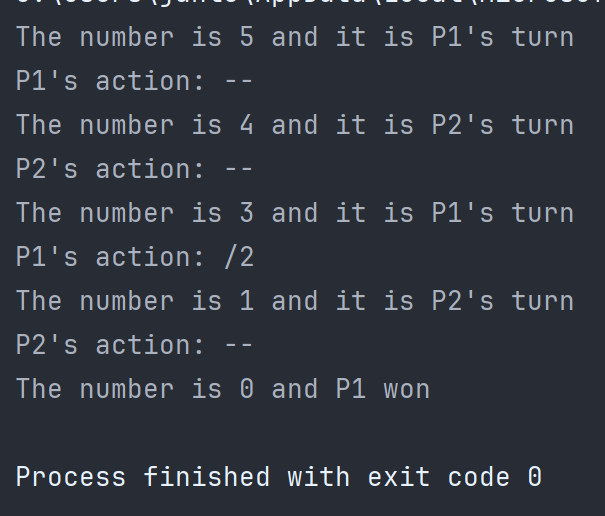
\includegraphics[width=0.8\textwidth]{Images/halving_game_terminal_output}
    \caption{Terminal output for a sample run of the halving game.}
    \label{fig:halving_game_terminal_output}
\end{figure}

\clearpage
\tcbsubtitle{The bucket game}

\begin{figure}[H]
    \centering
    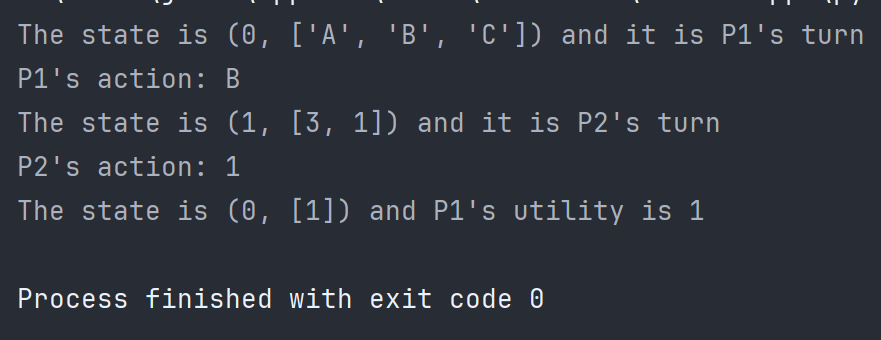
\includegraphics[width=0.8\textwidth]{Images/bucket_game}
    \caption{Terminal output for a sample run of the bucket game.}
    \label{fig:sudoku_easy}
\end{figure}

\clearpage
\tcbsubtitle{Tic-tac-toe}

\begin{figure}[H]
    \centering
    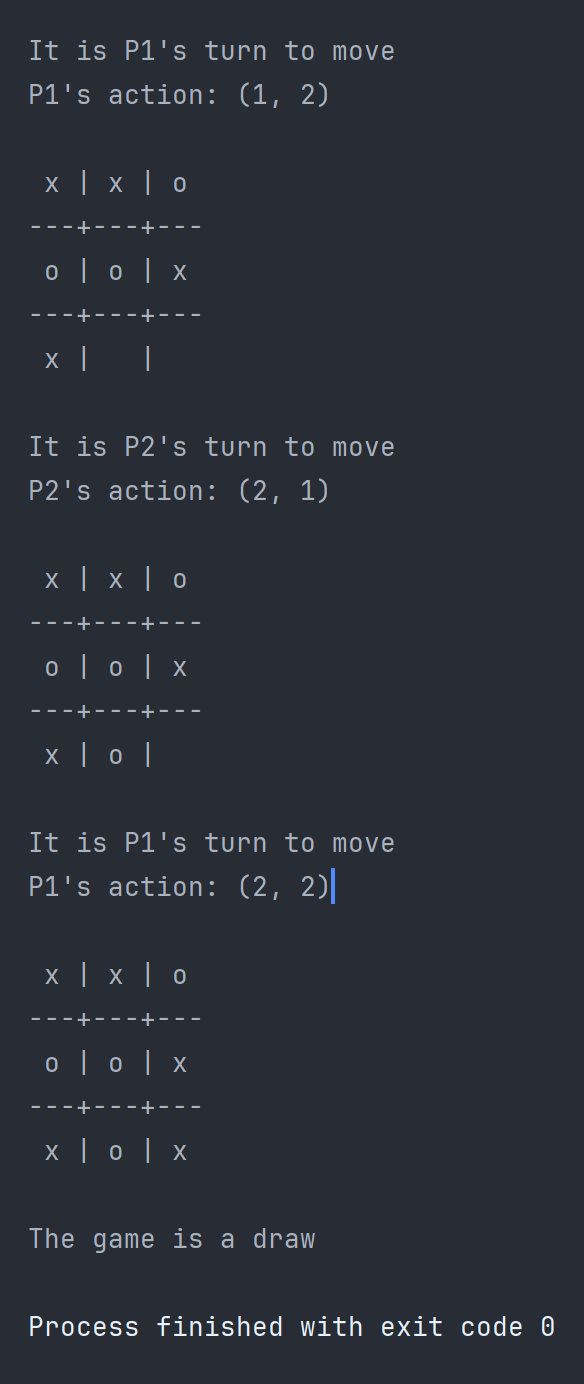
\includegraphics[width=0.5\textwidth]{Images/tic_tac_toe}
    \caption{Terminal output for a sample run of tic-tac-toe. This is not the entire output, as the game tree is quite large.}
    \label{fig:tic_tac_toe_terminal_output}
\end{figure}

\begin{figure}[H]
    \centering
    \begin{minipage}[b]{0.48\textwidth}
        \centering
        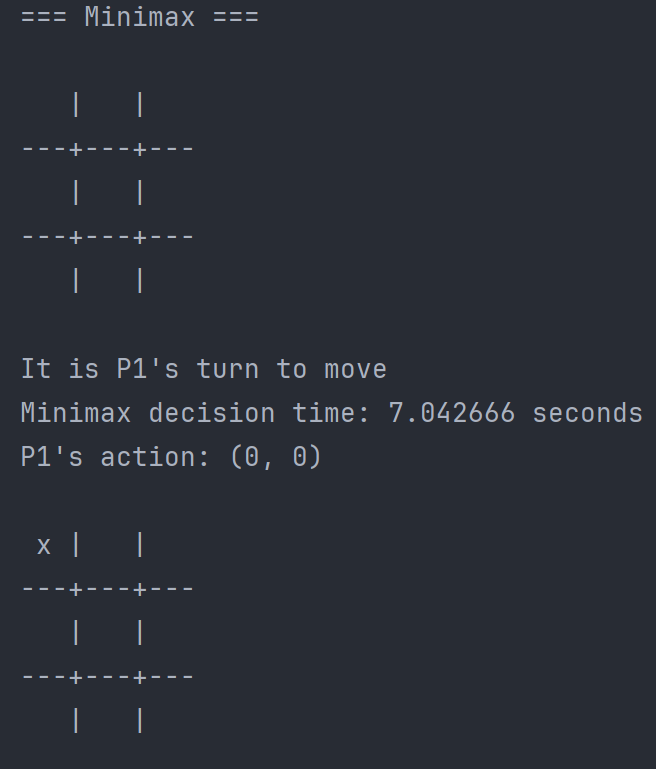
\includegraphics[width=\textwidth]{Images/tic_tac_toe_decision_time_minimax}
        \caption{Terminal output showing the decision time for the minimax algorithm for the first move.}
        \label{fig:tic_tac_toe_decision_time_minimax}
    \end{minipage}
    \hfill
    \begin{minipage}[b]{0.48\textwidth}
        \centering
        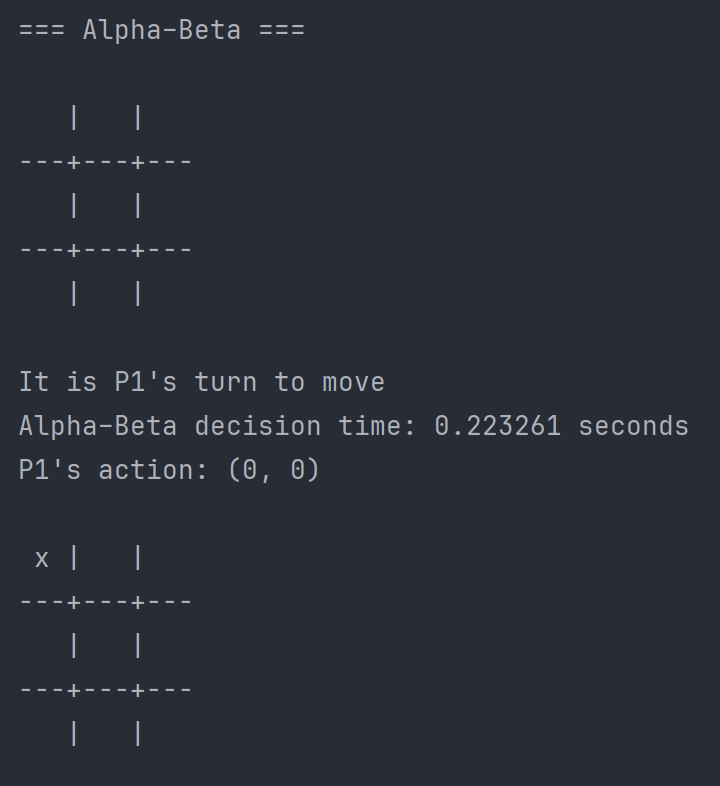
\includegraphics[width=\textwidth]{Images/tic_tac_toe_decision_time_alphabeta}
        \caption{Terminal output showing the decision time for the alpha--beta pruning for the first move.}
        \label{fig:tic_tac_toe_decision_time_alphabeta}
    \end{minipage}
\end{figure}

\end{document}
